\section{Preventivo}
Per facilitare la lettura delle seguenti tabelle, vengono utilizzate delle sigle 
per identificare i ruoli:
\begin{itemize}
\item \textbf{Re:} \textit{Responsabile};
\item \textbf{Ad:} \textit{Amministratore};
\item \textbf{An:} \textit{Analista};
\item \textbf{Pt:} \textit{Progettista};
\item \textbf{Pr:} \textit{Programmatore};
\item \textbf{Ve:} \textit{Verificatore}.
\end{itemize}
\noindent
Inoltre, se le ore ricoperte in un determinato ruolo fossero nulle, la cella 
presenterà il simbolo \textbf{-} per indicarne l'assenza. 

\subsection{Fase di Analisi}
\subsubsection{Prospetto orario}
In questa fase, ogni componente del gruppo rivestirà i seguenti ruoli:
\begin{table}[H]
		\begin{center}
			\setlength{\aboverulesep}{0pt}
			\setlength{\belowrulesep}{0pt}
			\setlength{\extrarowheight}{.75ex}
			\rowcolors{2}{AzzurroGruppo!10}{white}
			\begin{tabular}{ c c c c c c c c }
				\rowcolor{AzzurroGruppo!30} 
				\textbf{Nominativo} & \textbf{Re} & \textbf{Am} & \textbf{An} & \textbf{Pt} & \textbf{Pr} & \textbf{Ve} & \textbf{Ore Totali}  \\
				\toprule
				Albiero Davide      & -  & 5  & 15 & - & - & 10 & 30 \\
				Calgaro Giosuè      & -  & 8  & 17 & - & - & 5  & 30 \\
				De Marchi Francesco & 9  & 4  & 10 & - & - & 7  & 30\\
				Giacchetto Daniele  & 10 & -  & 10 & - & - & 10 & 30\\
				Gradi Lucrezia      & -  & 3 & 12 & - & - & 15 & 30\\
				Pagotto Matteo      & 5  & 5  & 10 & - & - & 10 & 30\\
				Poppi Tommaso       & 5  & 7  & 10 & - & - & 8  & 30\\
				 \textbf{Ore totali} & \textbf{29} & \textbf{32} & \textbf{84} & \textbf{-} & \textbf{-} & \textbf{65} & \textbf{210} \\
				\bottomrule
			\end{tabular}
			\caption{Distribuzione delle ore nel periodo di Analisi}
		\end{center}
	\end{table}
I dati ottenuti vengono riassunti nel seguente istogramma
\begin{figure}[H]
    \centering
    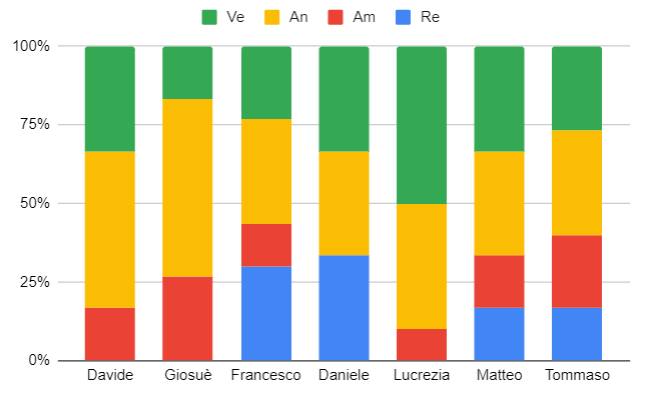
\includegraphics[scale = 0.5]{components/img/Analisi_isto.png}
    \caption{ Istogramma della ripartizione di ore per ruolo in Analisi}
    \label{fig:logo}
\end{figure}
\subsubsection{Prospetto economico}
Il costo per ogni ruolo è il seguente:
\begin{table}[H]
		\begin{center}
			\setlength{\aboverulesep}{0pt}
			\setlength{\belowrulesep}{0pt}
			\setlength{\extrarowheight}{.75ex}
			\rowcolors{2}{AzzurroGruppo!10}{white}
			\begin{tabular}{ c c c }
				\rowcolor{AzzurroGruppo!30} 
				\textbf{Ruolo} & \textbf{Ore} & \textbf{Costo}  \\
				\toprule
				Responsabile & 29 & 870€ \\
				Amministratore & 32 & 640€ \\
				Analista & 84 & 2100€ \\
				Progettista & - & - \\
				Programmatore & - & - \\
				Verificatore & 65 & 975€ \\
				\textbf{Totale} & \textbf{210} & \textbf{4585€} \\
				\bottomrule
			\end{tabular}
			\caption{ Prospetto dei costi per ruoli nel periodo di Analisi}
		\end{center}
\end{table}
I dati ottenuti si posoono riassumere nel seguente aerogramma:
\begin{figure}[H]
    \centering
    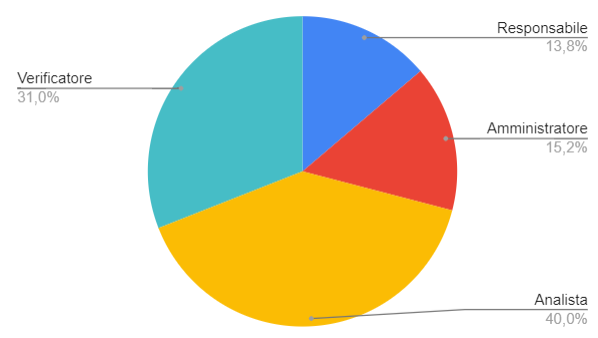
\includegraphics[scale = 0.5]{components/img/analisi_torta.png}
    \caption{ Areogramma della ripartizione di ore per ruolo in Analisi}
    \label{fig:logo}
\end{figure}
\subsection{Fase di consolidamento dei requisiti}
\subsubsection{Prospetto orario}
durante il periodo di consolidamento dei requisiti viene effettuata la seguente distribuzione oraria:
\begin{table}[H]
		\begin{center}
			\setlength{\aboverulesep}{0pt}
			\setlength{\belowrulesep}{0pt}
			\setlength{\extrarowheight}{.75ex}
			\rowcolors{2}{AzzurroGruppo!10}{white}
			\begin{tabular}{ c c c c c c c c }
				\rowcolor{AzzurroGruppo!30} 
				\textbf{Nominativo} & \textbf{Re} & \textbf{Am} & \textbf{An} & \textbf{Pt} & \textbf{Pr} & \textbf{Ve} & \textbf{Ore Totali}  \\
				\toprule
				Albiero Davide      & - & - & 3 & - & - & 2 & 5 \\
				Calgaro Giosuè      & - & - & - & - & - & 5 & 5 \\
				De Marchi Francesco & - & - & 5 & - & - & - & 5\\
				Giacchetto Daniele  & - & 3 & - & - & - & 2 & 5\\
				Gradi Lucrezia      & 3 & - & - & - & - & 2 & 5\\
				Pagotto Matteo      & - & - & 5 & - & - & - & 5\\
				Poppi Tommaso       & - & - & 3 & - & - & 2 & 5\\
				 \textbf{Ore totali} & \textbf{3} & \textbf{3} & \textbf{16} & \textbf{-} & \textbf{-} & \textbf{13} & \textbf{35} \\
				\bottomrule
			\end{tabular}
			\caption{Distribuzione delle ore nel periodo di Consolidamento dei requisiti}
		\end{center}
	\end{table}
I dati ottenuti vengono riassunti nel seguente istogramma:
\begin{figure}[H]
    \centering
    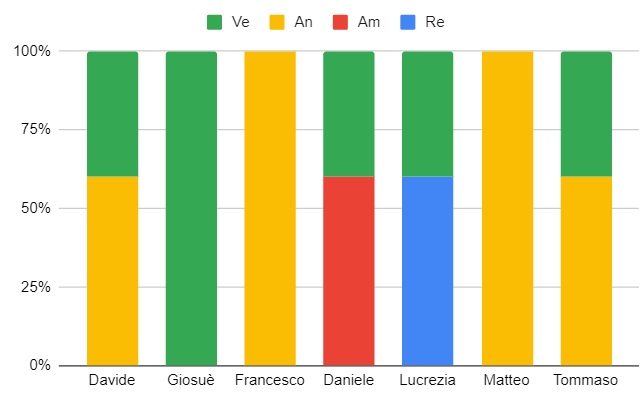
\includegraphics[scale = 0.5]{components/img/consolidamento_isto.png}
    \caption{Istogramma della ripartizione di ore per ruolo in Consolidamento dei requisiti}
    \label{fig:logo}
\end{figure}
\subsubsection{Prospetto economico}
Il costo per ogni ruolo è il seguente:
\begin{table}[H]
		\begin{center}
			\setlength{\aboverulesep}{0pt}
			\setlength{\belowrulesep}{0pt}
			\setlength{\extrarowheight}{.75ex}
			\rowcolors{2}{AzzurroGruppo!10}{white}
			\begin{tabular}{ c c c }
				\rowcolor{AzzurroGruppo!30} 
				\textbf{Ruolo} & \textbf{Ore} & \textbf{Costo}  \\
				\toprule
				Responsabile   & 3 & 90€ \\
				Amministratore & 3 & 60€ \\
				Analista       & 16 & 400€ \\
				Progettista    & - & - \\
				Programmatore  & - & - \\
				Verificatore   & 13 & 195€ \\
				\textbf{Totale} & \textbf{35} & \textbf{745€} \\
				\bottomrule
			\end{tabular}
			\caption{ Prospetto dei costi per ruoli nel periodo di Consolidamento dei requisiti}
		\end{center}
	\end{table}
I dati ottenuti si posoono riassumere nel seguente aerogramma:
\begin{figure}[H]
    \centering
    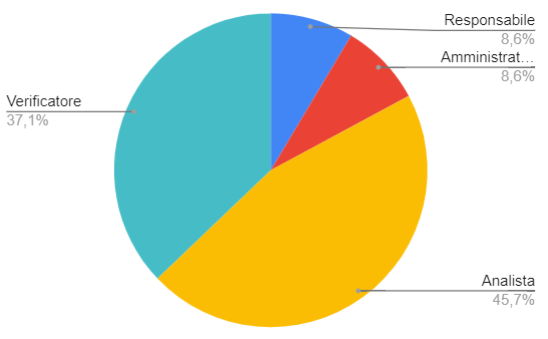
\includegraphics[scale = 0.5]{components/img/consolidamento_torta.png}
    \caption{ Areogramma della ripartizione di ore per ruolo in Consolidamento dei Requisiti}
    \label{fig:logo}
\end{figure}
\subsection{Fase di Progettazione architetturale}
\subsubsection{Prospetto orario}
In questa fase la distribuzione oraria è la seguente:
\begin{table}[H]
		\begin{center}
			\setlength{\aboverulesep}{0pt}
			\setlength{\belowrulesep}{0pt}
			\setlength{\extrarowheight}{.75ex}
			\rowcolors{2}{AzzurroGruppo!10}{white}
			\begin{tabular}{ c c c c c c c c }
				\rowcolor{AzzurroGruppo!30} 
				\textbf{Nominativo} & \textbf{Re} & \textbf{Am} & \textbf{An} & \textbf{Pt} & \textbf{Pr} & \textbf{Ve} & \textbf{Ore Totali}  \\
				\toprule
				Albiero Davide      & 5  & 6 & -  & -  & 4 & 15 & 30 \\
				Calgaro Giosuè      & 3  & - & -  & 16 & 5 & 6  & 30 \\
				De Marchi Francesco & -  & - & 8  & 12 & 3 & 7  & 30\\
				Giacchetto Daniele  & -  & 3 & 10 & 13 & - & 4  & 30\\
				Gradi Lucrezia      & -  & - & 10 & -  & 4 & 16 & 30\\
				Pagotto Matteo      & 10 & 8 & -  & 12 & - & -  & 30\\
				Poppi Tommaso       & -  & 3 & 10 & 8  & 5 & 4  & 30\\
				 \textbf{Ore totali} & \textbf{18} & \textbf{20} & \textbf{38} & \textbf{61} & \textbf{21} & \textbf{52} & \textbf{210} \\
				\bottomrule
			\end{tabular}
			\caption{Distribuzione delle ore nel periodo di  Progettazione architetturale}
		\end{center}
	\end{table}
I dati ottenuti vengono riassunti nel seguente istogramma:
\begin{figure}[H]
    \centering
    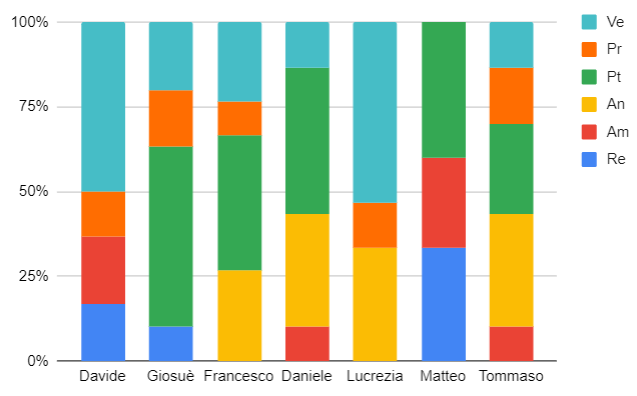
\includegraphics[scale = 0.5]{components/img/architettura_isto.png}
    \caption{Istogramma della ripartizione di ore per ruolo in Progettazione architetturale}
    \label{fig:logo}
\end{figure}
\subsubsection{Prospetto economico}
Il costo per ogni ruolo è il seguente:
\begin{table}[H]
		\begin{center}
			\setlength{\aboverulesep}{0pt}
			\setlength{\belowrulesep}{0pt}
			\setlength{\extrarowheight}{.75ex}
			\rowcolors{2}{AzzurroGruppo!10}{white}
			\begin{tabular}{ c c c }
				\rowcolor{AzzurroGruppo!30} 
				\textbf{Ruolo} & \textbf{Ore} & \textbf{Costo}  \\
				\toprule
				Responsabile   & 18 & 540€ \\
				Amministratore & 20 & 400€ \\
				Analista       & 38 & 950€ \\
				Progettista    & 61 & 1342€ \\
				Programmatore  & 21 & 315€ \\
				Verificatore   & 52 & 780€ \\
				\textbf{Totale} & \textbf{210} & \textbf{4327€} \\
				\bottomrule
			\end{tabular}
			\caption{ Prospetto dei costi per ruoli nel periodo di Progettazione architetturale}
		\end{center}
	\end{table}
I dati ottenuti si posoono riassumere nel seguente aerogramma:
\begin{figure}[H]
    \centering
    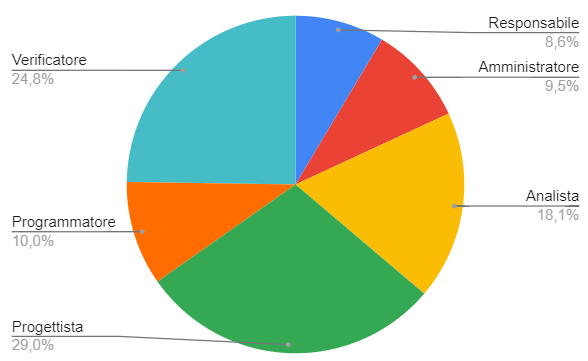
\includegraphics[scale = 0.5]{components/img/architettura_torta.png}
    \caption{ Areogramma della ripartizione di ore per ruolo in Progettazione architetturale}
    \label{fig:logo}
\end{figure}
\subsection{Fase di Progettazione di dettaglio e codifica}
\subsubsection{Prospetto orario}
in questa fase la distribuzione oraria è la seguente
\begin{table}[H]
		\begin{center}
			\setlength{\aboverulesep}{0pt}
			\setlength{\belowrulesep}{0pt}
			\setlength{\extrarowheight}{.75ex}
			\rowcolors{2}{AzzurroGruppo!10}{white}
			\begin{tabular}{ c c c c c c c c }
				\rowcolor{AzzurroGruppo!30} 
				\textbf{Nominativo} & \textbf{Re} & \textbf{Am} & \textbf{An} & \textbf{Pt} & \textbf{Pr} & \textbf{Ve} & \textbf{Ore Totali}  \\
				\toprule
				Albiero Davide      & - & - & - & 15 & 20 & 15 & 50 \\
				Calgaro Giosuè      & 5 & 2 & - & 6 & 20 & 17 & 50 \\
				De Marchi Francesco & 4 & 4 & - & 12 & 20 & 10 & 50 \\
				Giacchetto Daniele  & - & - & - & 15 & 20 & 15 & 50 \\
				Gradi Lucrezia      & - & 8 & - & 15 & 15 & 12 & 50 \\
				Pagotto Matteo      & 4 & - & - & 15 & 21 & 10 & 50 \\
				Poppi Tommaso       & 5 & 4 & - & 11 & 18 & 12 & 50 \\
				 \textbf{Ore totali} & \textbf{18} & \textbf{18} & \textbf{-} & \textbf{89} & \textbf{134} & \textbf{91} & \textbf{350} \\
				\bottomrule
			\end{tabular}
			\caption{Distribuzione delle ore nel periodo di Progettazione di dettaglio e codifica}
		\end{center}
	\end{table}
	I dati ottenuti vengono riassunti nel seguente istogramma:
\begin{figure}[H]
    \centering
    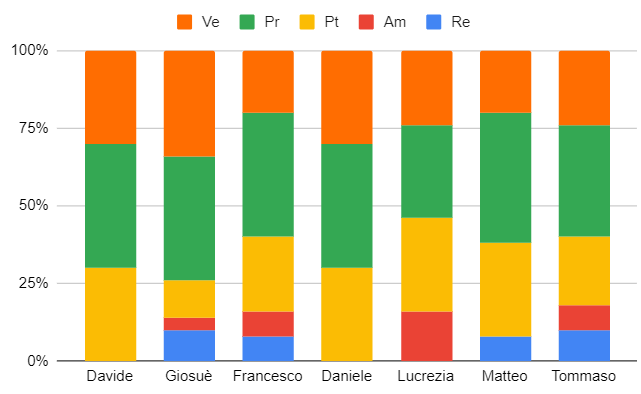
\includegraphics[scale = 0.5]{components/img/dettaglio_isto.png}
    \caption{Istogramma della ripartizione di ore per ruolo in Progettazione di dettaglio e codifica}
    \label{fig:logo}
\end{figure}
\subsubsection{Prospetto economico}
Il costo per ogni ruolo è il seguente:
\begin{table}[H]
		\begin{center}
			\setlength{\aboverulesep}{0pt}
			\setlength{\belowrulesep}{0pt}
			\setlength{\extrarowheight}{.75ex}
			\rowcolors{2}{AzzurroGruppo!10}{white}
			\begin{tabular}{ c c c }
				\rowcolor{AzzurroGruppo!30} 
				\textbf{Ruolo} & \textbf{Ore} & \textbf{Costo}  \\
				\toprule
				Responsabile   & 18 & 540€ \\
				Amministratore & 18 & 360€ \\
				Analista       & - & - \\
				Progettista    & 89 & 1958€ \\
				Programmatore  & 134 & 2010€ \\
				Verificatore   & 91 & 1365€ \\
				\textbf{Totale} & \textbf{350} & \textbf{6233€} \\
				\bottomrule
			\end{tabular}
			\caption{ Prospetto dei costi per ruoli nel periodo di Progettazione di dettaglio e codifica}
		\end{center}
	\end{table}
I dati ottenuti si posoono riassumere nel seguente aerogramma:
\begin{figure}[H]
    \centering
    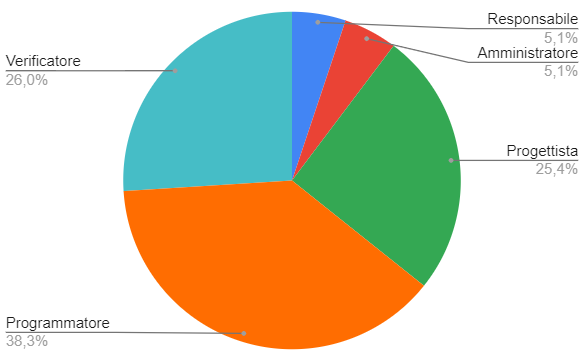
\includegraphics[scale = 0.5]{components/img/dettaglio_torta.png}
    \caption{ Areogramma della ripartizione di ore per ruolo in Progettazione di dettaglio e codifica}
    \label{fig:logo}
\end{figure}
\subsection{Fase di Validazione e collaudo}
\subsubsection{Prospetto orario}
in questa fase la distribuzione oraria è la seguente
\begin{table}[H]
		\begin{center}
			\setlength{\aboverulesep}{0pt}
			\setlength{\belowrulesep}{0pt}
			\setlength{\extrarowheight}{.75ex}
			\rowcolors{2}{AzzurroGruppo!10}{white}
			\begin{tabular}{ c c c c c c c c }
				\rowcolor{AzzurroGruppo!30} 
				\textbf{Nominativo} & \textbf{Re} & \textbf{Am} & \textbf{An} & \textbf{Pt} & \textbf{Pr} & \textbf{Ve} & \textbf{Ore Totali}  \\
				\toprule
				Albiero Davide      & 4 & 5 & - & - & 5 & 6 & 20 \\
				Calgaro Giosuè      & - & - & - & 4 & 6 & 10 & 20 \\
				De Marchi Francesco & - & 6 & - & - & 8 & 6 & 20\\
				Giacchetto Daniele  & 4 & - & - & - & 4 & 12 & 20\\
				Gradi Lucrezia      & 5 & - & - & - & 7 & 8 & 20\\
				Pagotto Matteo      & 4 & - & - & - & 6 & 10 & 20\\
				Poppi Tommaso       & - & 5 & - & 5 & - & 10 & 20\\
				 \textbf{Ore totali} & \textbf{17} & \textbf{16} & \textbf{-} & \textbf{9} & \textbf{36} & \textbf{62} & \textbf{140} \\
				\bottomrule
			\end{tabular}
			\caption{Distribuzione delle ore nel periodo di Validazione e collaudo}
		\end{center}
	\end{table}
	I dati ottenuti vengono riassunti nel seguente istogramma:
	\begin{figure}[H]
    \centering
    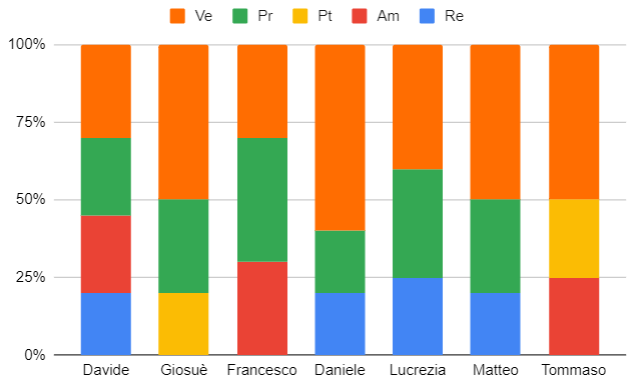
\includegraphics[scale = 0.5]{components/img/validazione_isto.png}
    \caption{Istogramma della ripartizione di ore per ruolo in Validazione e collaudo}
    \label{fig:logo}
\end{figure}
\subsubsection{Prospetto economico}
Il costo per ogni ruolo è il seguente:
\begin{table}[H]
		\begin{center}
			\setlength{\aboverulesep}{0pt}
			\setlength{\belowrulesep}{0pt}
			\setlength{\extrarowheight}{.75ex}
			\rowcolors{2}{AzzurroGruppo!10}{white}
			\begin{tabular}{ c c c }
				\rowcolor{AzzurroGruppo!30} 
				\textbf{Ruolo} & \textbf{Ore} & \textbf{Costo}  \\
				\toprule
				Responsabile   & 17 & 510€ \\
				Amministratore & 16 & 320€ \\
				Analista       & -  & - \\
				Progettista    & 9  & 198€ \\
				Programmatore  & 36 & 540€ \\
				Verificatore   & 62 & 930€ \\
				\textbf{Totale} & \textbf{140} & \textbf{2498€} \\
				\bottomrule
			\end{tabular}
			\caption{ Prospetto dei costi per ruoli nel periodo di Validazione e collaudo}
		\end{center}
	\end{table}
I dati ottenuti si posoono riassumere nel seguente aerogramma:
\begin{figure}[H]
    \centering
    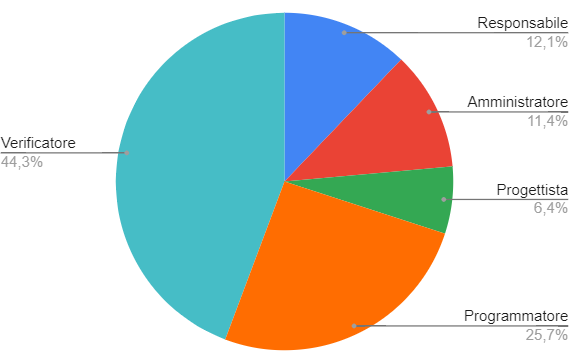
\includegraphics[scale = 0.5]{components/img/validazione_torta.png}
    \caption{ Areogramma della ripartizione di ore per ruolo in Validazione e collaudo}
    \label{fig:logo}
\end{figure}
\subsection{Riepilogo}
\subsubsection{Ore totali}
\paragraph{Suddivisione del lavoro}
Nella seguente tabella vengono riportate il totale delle ore del progetto, sono presenti sia le ore di investimento, sia le ore rendicontate a carico del committente.
\begin{table}[H]
		\begin{center}
			\setlength{\aboverulesep}{0pt}
			\setlength{\belowrulesep}{0pt}
			\setlength{\extrarowheight}{.75ex}
			\rowcolors{2}{AzzurroGruppo!10}{white}
			\begin{tabular}{ c c c c c c c c }
				\rowcolor{AzzurroGruppo!30} 
				\textbf{Nominativo} & \textbf{Re} & \textbf{Am} & \textbf{An} & \textbf{Pt} & \textbf{Pr} & \textbf{Ve} & \textbf{Ore Totali}  \\
				\toprule
				Albiero Davide      & 9 & 16 & 18 & 15 & 29 & 48 & 135 \\
				Calgaro Giosuè      & 8 & 10 & 17 & 26 & 31 & 43 & 135 \\
				De Marchi Francesco & 13 & 14 & 23 & 24 & 31 & 30 & 135\\
				Giacchetto Daniele  & 14 & 6 & 20 & 28 & 24 & 43 & 135\\
				Gradi Lucrezia      & 8 & 11 & 22 & 15 & 26 & 53 & 135\\
				Pagotto Matteo      & 23 & 13 & 15 & 27 & 27 & 30 & 135\\
				Poppi Tommaso       & 10 & 19 & 23 & 24 & 23 & 36 & 135\\
				 \textbf{Ore totali} & \textbf{76} & \textbf{73} & \textbf{120} & \textbf{144} & \textbf{162} & \textbf{235} & \textbf{945} \\
				\bottomrule
			\end{tabular}
			\caption{ Distribuzione delle ore totali di investimento e rendicontate}
		\end{center}
	\end{table}
	I dati ottenuti vengono riassunti nel seguente istogramma:
\begin{figure}[H]
    \centering
    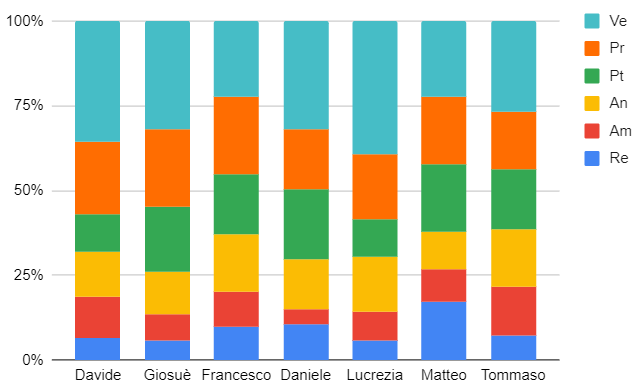
\includegraphics[scale = 0.5]{components/img/totale_isto.png}
    \caption{ Istogramma della ripartizione di ore totali di investimento e rendicontate}
    \label{fig:logo}
\end{figure}
\paragraph{Prospetto economico}
Il costo per ogni ruolo è il seguente:
\begin{table}[H]
		\begin{center}
			\setlength{\aboverulesep}{0pt}
			\setlength{\belowrulesep}{0pt}
			\setlength{\extrarowheight}{.75ex}
			\rowcolors{2}{AzzurroGruppo!10}{white}
			\begin{tabular}{ c c c }
				\rowcolor{AzzurroGruppo!30} 
				\textbf{Ruolo} & \textbf{Ore} & \textbf{Costo}  \\
				\toprule
				Responsabile   & 85 & 2550€ \\
				Amministratore & 89 & 1780€ \\
				Analista       & 138 & 3450€ \\
				Progettista    & 159 & 3498€ \\
				Programmatore  & 191 & 2865€ \\
				Verificatore   & 283 & 4245€ \\
				\textbf{Totale} & \textbf{945} & \textbf{18388€} \\
				\bottomrule
			\end{tabular}
			\caption{ Prospetto dei costi totale delle ore di investimento e rendicontate}
		\end{center}
	\end{table}
I dati ottenuti si posoono riassumere nel seguente aerogramma:
\begin{figure}[H]
    \centering
    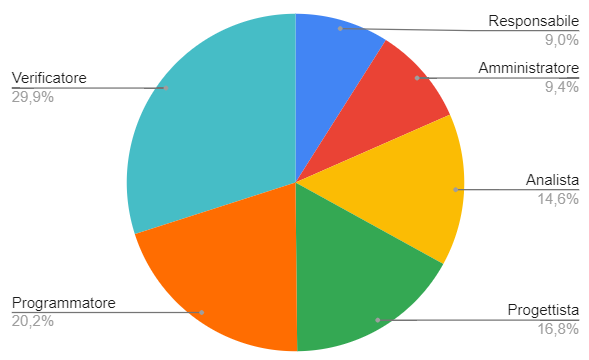
\includegraphics[scale = 0.5]{components/img/tot_torta.png}
    \caption{ Areogramma dei costi totale delle ore di investimento e rendicontate}
    \label{fig:logo}
\end{figure}
\subsubsection{Ore rendicontate}
\paragraph{Suddivisione del lavoro}
Nella seguente tabella sono riassunte le ore rendicontate:
\begin{table}[H]
		\begin{center}
			\setlength{\aboverulesep}{0pt}
			\setlength{\belowrulesep}{0pt}
			\setlength{\extrarowheight}{.75ex}
			\rowcolors{2}{AzzurroGruppo!10}{white}
			\begin{tabular}{ c c c c c c c c }
				\rowcolor{AzzurroGruppo!30} 
				\textbf{Nominativo} & \textbf{Re} & \textbf{Am} & \textbf{An} & \textbf{Pt} & \textbf{Pr} & \textbf{Ve} & \textbf{Ore Totali}  \\
				\toprule
				Albiero Davide      & 9  & 11 & -  & 15  & 29 & 36 & 100 \\
				Calgaro Giosuè      & 8  & 2 & -  & 26 & 31 & 33  & 100 \\
				De Marchi Francesco & 4  & 10 & 8  & 24 & 31 & 23  & 100\\
				Giacchetto Daniele  & 4  & 3 & 10 & 28 & 24 & 31  & 100\\
				Gradi Lucrezia      & 5  & 8 & 10 & 15  & 26 & 36 & 100\\
				Pagotto Matteo      & 18 & 8 & -  & 27 & 27 & 20  & 100\\
				Poppi Tommaso       & 5  & 12 & 10 & 24  & 23 & 26  & 100\\
				 \textbf{Ore totali} & \textbf{53} & \textbf{54} & \textbf{38} & \textbf{159} & \textbf{191} & \textbf{205} & \textbf{700} \\
				\bottomrule
			\end{tabular}
			\caption{Distribuzione delle ore rendicontate}
		\end{center}
	\end{table}
	I dati ottenuti vengono riassunti nel seguente istogramma:
\begin{figure}[H]
    \centering
    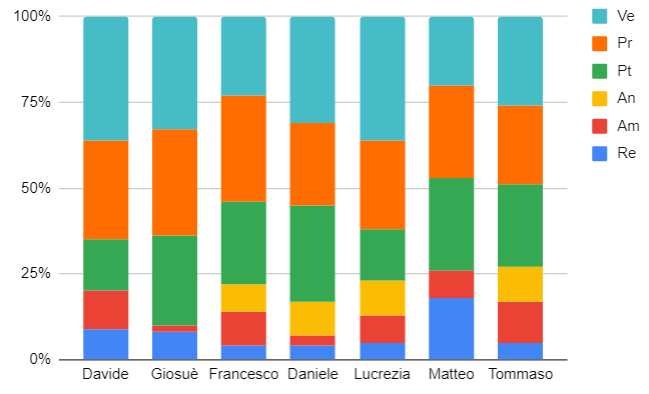
\includegraphics[scale = 0.5]{components/img/rendiconto_isto.png}
    \caption{ Istogramma della ripartizione delle ore rendicontate}
    \label{fig:logo}
\end{figure}
\paragraph{Prospetto economico}
Il costo totale rendicontato per ogni ruolo è il seguente:
\begin{table}[H]
		\begin{center}
			\setlength{\aboverulesep}{0pt}
			\setlength{\belowrulesep}{0pt}
			\setlength{\extrarowheight}{.75ex}
			\rowcolors{2}{AzzurroGruppo!10}{white}
			\begin{tabular}{ c c c }
				\rowcolor{AzzurroGruppo!30} 
				\textbf{Ruolo} & \textbf{Ore} & \textbf{Costo}  \\
				\toprule
				Responsabile   & 58 & 1590€ \\
				Amministratore & 54 & 1080€ \\
				Analista       & 38 & 950€ \\
				Progettista    & 159 & 2865€ \\
				Programmatore  & 191 & 3075€ \\
				Verificatore   & 205 & 3075€ \\
				\textbf{Totale} & \textbf{700} & \textbf{13058€} \\
				\bottomrule
			\end{tabular}
			\caption{Prospetto dei costi delle ore rendicontate}
		\end{center}
	\end{table}
I dati ottenuti si possono riassumere nel seguente aerogramma:
\begin{figure}[H]
    \centering
    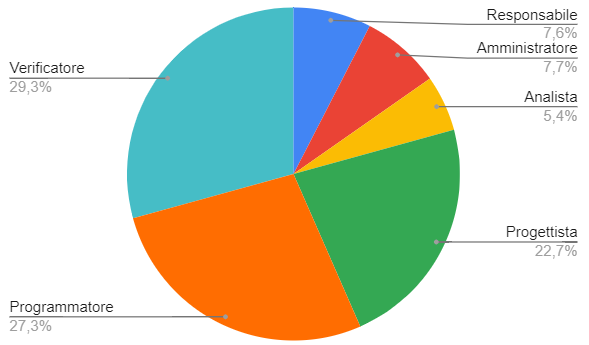
\includegraphics[scale = 0.5]{components/img/rendiconto_torta.png}
    \caption{Areogramma delle ore rendicontate per ruolo}
    \label{fig:logo}
\end{figure}
\subsubsection{Conclusioni}
il costo totale preventivato è : 13058€ .